
%%%%%%%%%%%%%%%%%%%%%%%%%%%%%%%%%%%%%%%%%%%%%%%%%%%%%%%%%%%%%
% %%%% 自己紹介スライド
%%%%%%%%%%%%%%%%%%%%%%%%%%%%%%%%%%%%%%%%%%%%%%%%%%%%%%%%%%%%%


%%%%%%%%%%%%%%%%%%%%%%%%%%%%%%%%%%%%%%
% 自己紹介
%%%%%%%%%%%%%%%%%%%%%%%%%%%%%%%%%%%%%%
\captionsetup[figure]{labelformat=empty,labelsep=none}
\begin{frame}
    \frametitle{自己紹介}
    \begin{itemize}
        \item 出身地\\
            三重県津市
        \item 好きなこと\\
            ドライブ,料理
        \item 趣味\\
            ゲーム,サイクリング,キャンプ
        \item 所属サークル\\
            名古屋大学アマチュア無線研究会
    \end{itemize}
    \begin{columns}
        \begin{column}{0.48\textwidth}
            \begin{figure}[htbp]
                \begin{center}
                    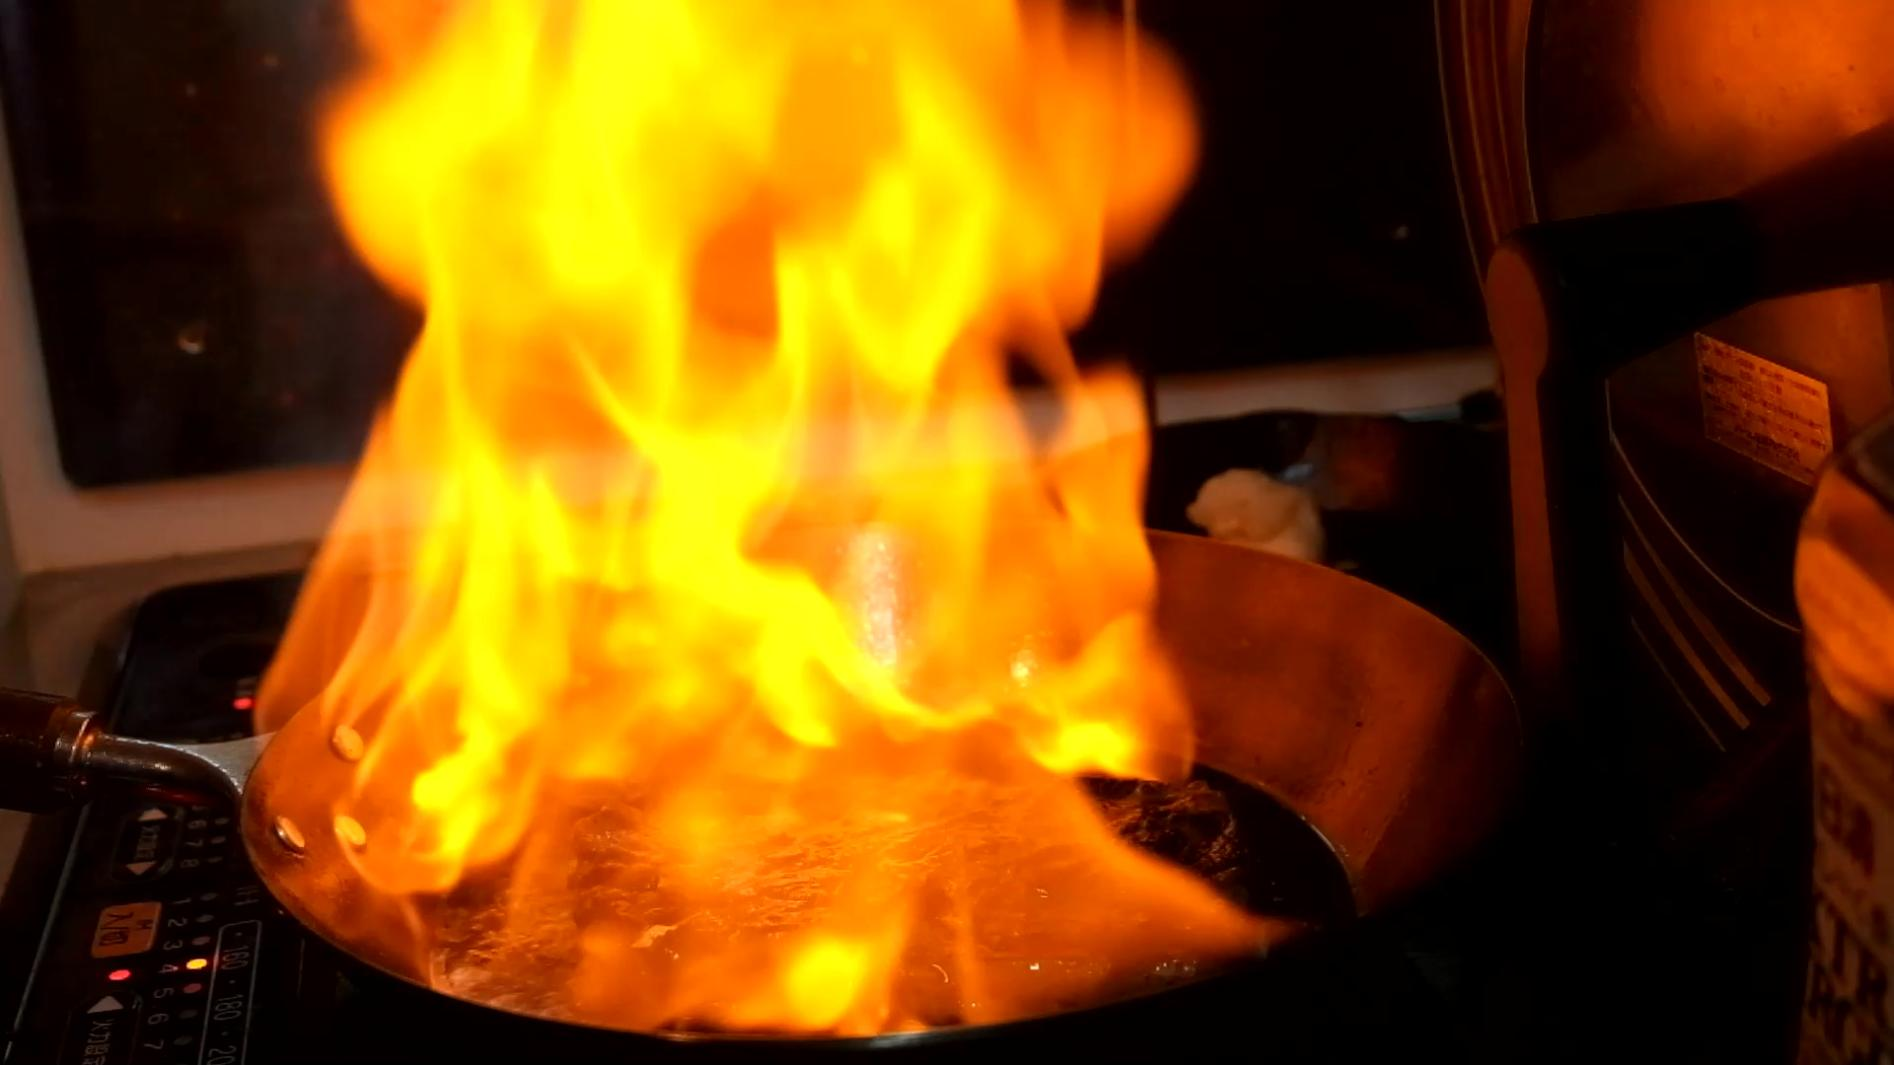
\includegraphics[width=50mm]{pic/pic1.jpg}
                \end{center}
                \caption{下宿先でフランベする図}
                % \label{fig:pic1}
            \end{figure}
        \end{column}
        \begin{column}{0.48\textwidth}
            \begin{figure}[htbp]
                \begin{center}
                    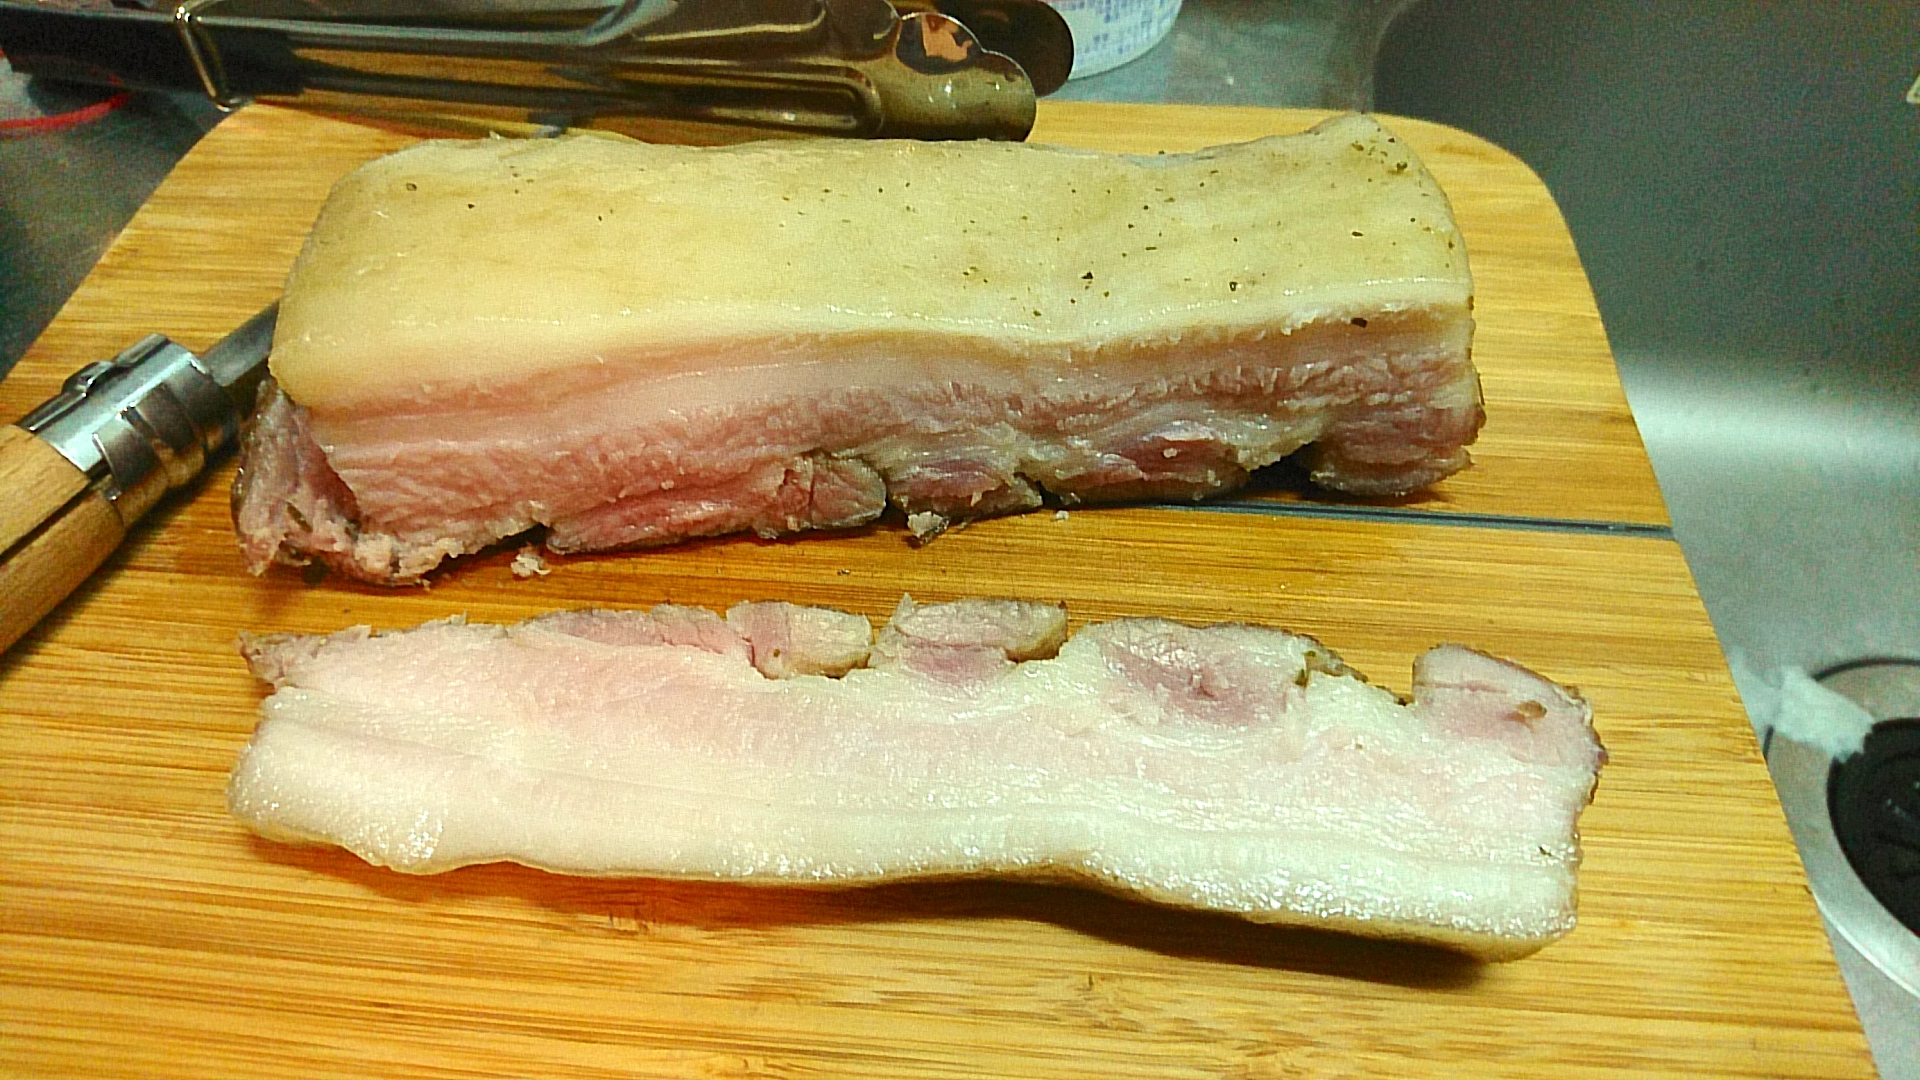
\includegraphics[width=50mm]{pic/pic2.jpg}
                \end{center}
                \caption{自家製ベーコン}
                % \label{fig:pic2}
            \end{figure}
        \end{column}
    \end{columns}
\end{frame}

%%%%%%%%%%%%%%%%%%%%%%%%%%%%%%%%%%%%%%
% 趣味:サイクリング
%%%%%%%%%%%%%%%%%%%%%%%%%%%%%%%%%%%%%%
\begin{frame}
    \frametitle{サイクリング}
    \begin{itemize}
        \item コロナ禍でドライブに行けなかったため,一人で誰にも迷惑をかけず遠くに行きたいと思い,卒論発表後にロードバイクを購入したことがきっかけで始めた.
        \item 今まで行った中で一番遠いところは,岐阜県恵那市(片道約60km)
        \item 1日での最高走行距離は約70km(常滑市まで往復)
    \end{itemize}
    \begin{block}{今後の目標}
        \begin{itemize}
            \item 実家(片道約60km)まで自転車で帰省する.
            \item 琵琶湖をキャンプしながら自転車で一周する
        \end{itemize}
    \end{block}
\end{frame}

%%%%%%%%%%%%%%%%%%%%%%%%%%%%%%%%%%%%%%
% 趣味:キャンプ
%%%%%%%%%%%%%%%%%%%%%%%%%%%%%%%%%%%%%%
\begin{frame}
    \frametitle{キャンプ}
    \begin{itemize}
        \item youtubeで見たブッシュクラフトの動画とアニメ"ゆるキャン△"がきっかけで始めた.
        \item 2018年のアマチュア無線コンテストの時に初めてキャンプをした.
        \item 最近までキャンプ道具を集めるだけになっていた.
        \item ロードバイクを買ったので,キャンプツーリングに行けるようになった.
    \end{itemize}
    \begin{columns}
        \begin{column}{0.48\textwidth}
            \begin{figure}[htbp]
                \begin{center}
                    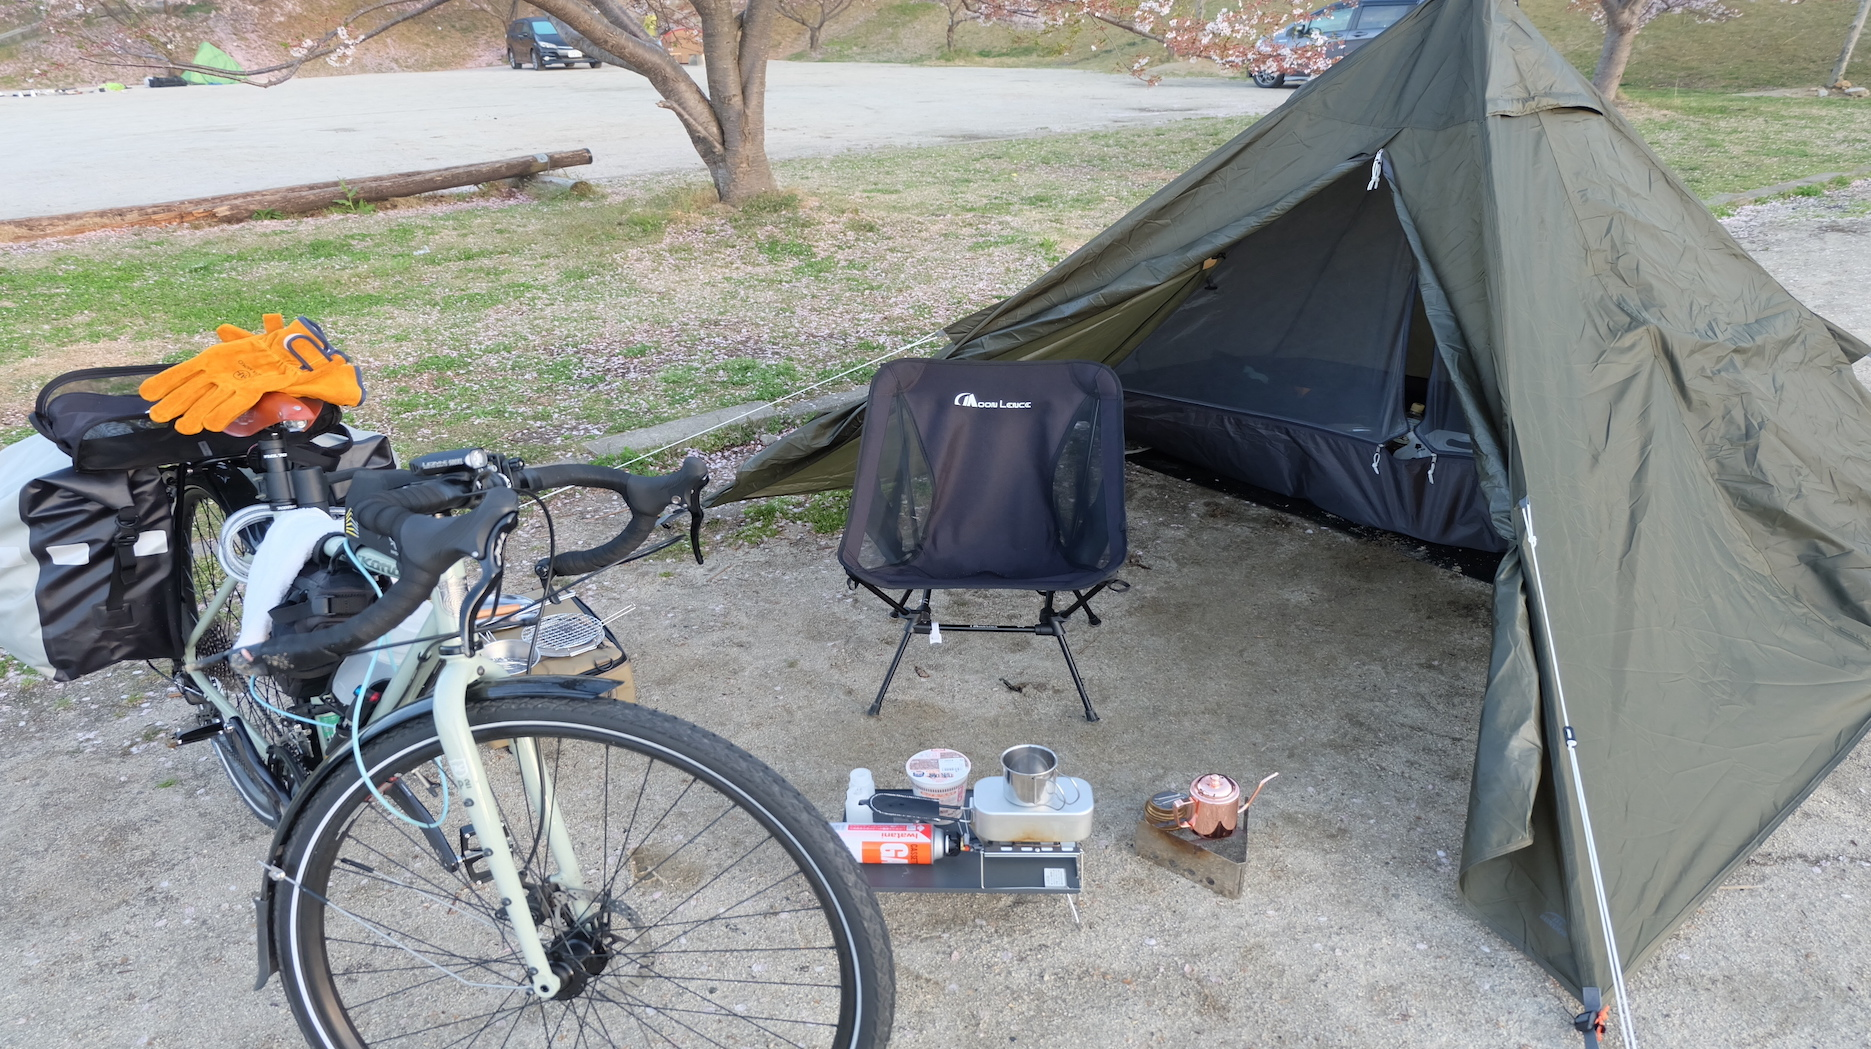
\includegraphics[width=50mm]{pic/pic3.JPG}
                \end{center}
                % \caption{下宿先でフランベする図}
                % \label{fig:pic1}
            \end{figure}
        \end{column}
        \begin{column}{0.48\textwidth}
            \begin{figure}[htbp]
                \begin{center}
                    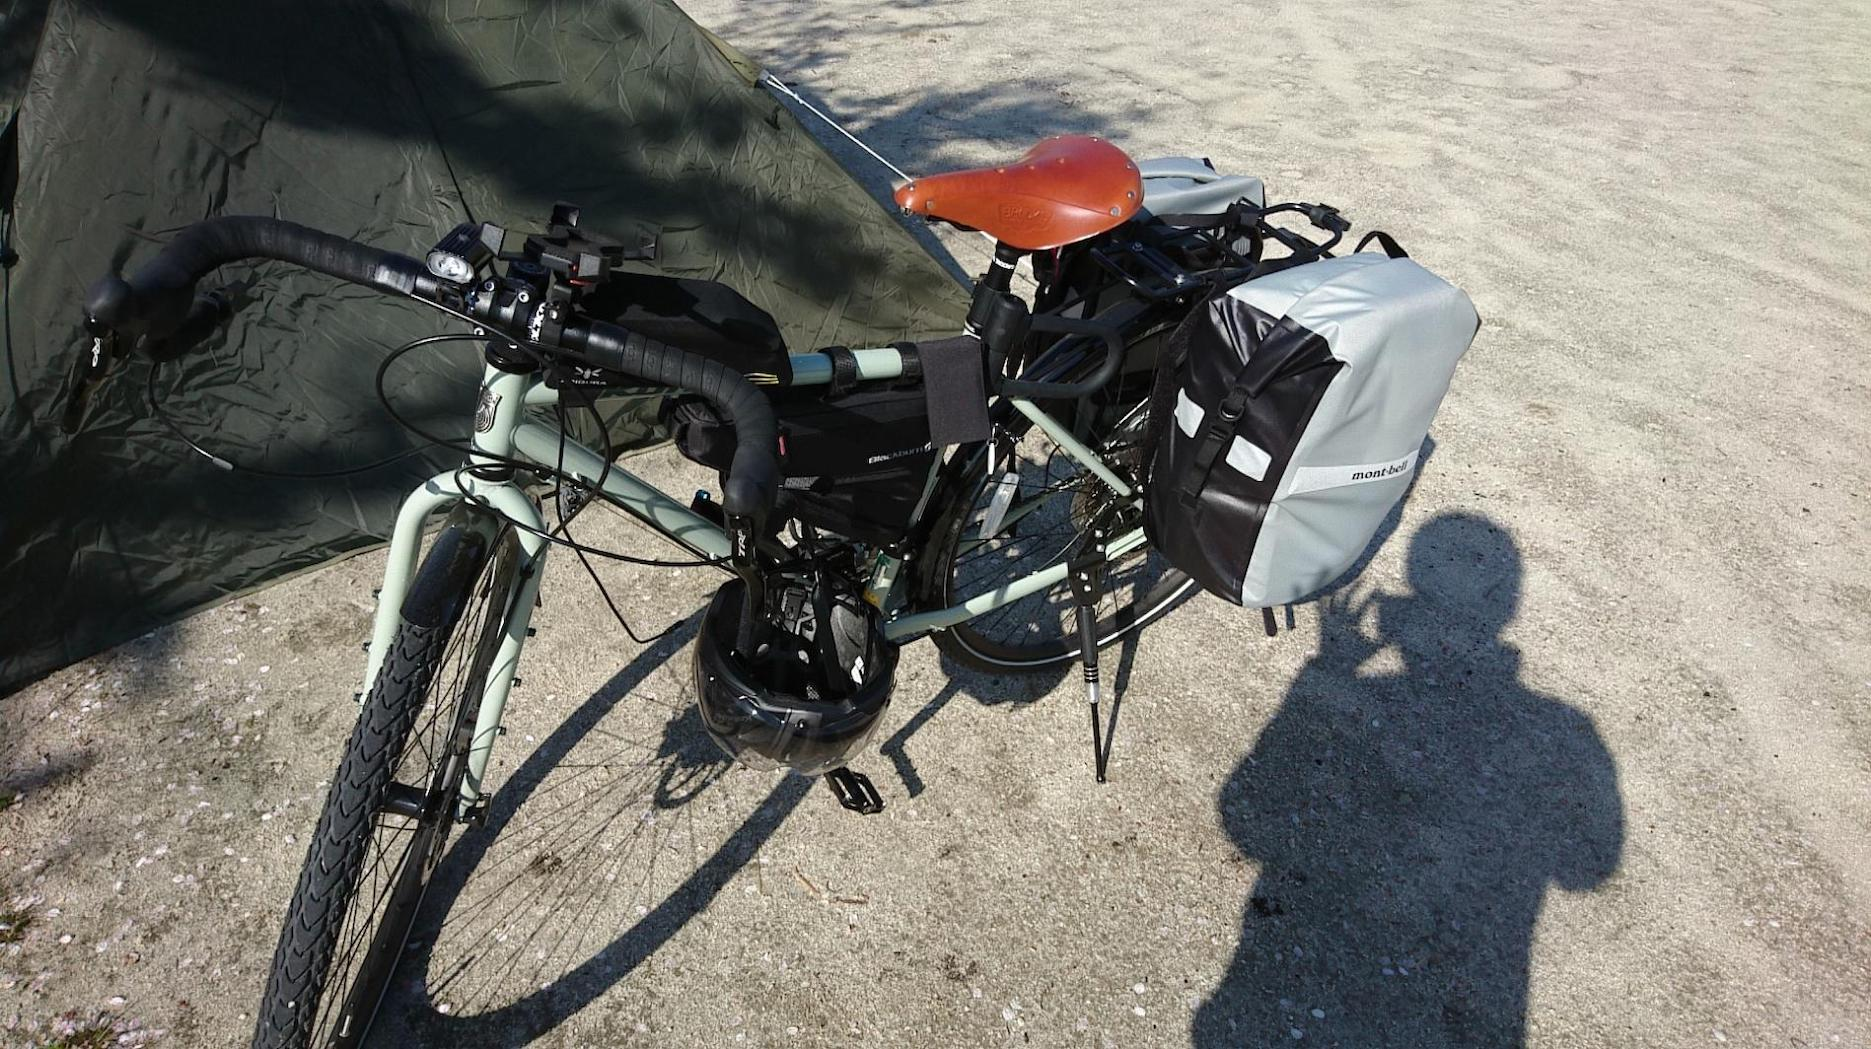
\includegraphics[width=50mm]{pic/pic4.JPG}
                \end{center}
                % \caption{自家製ベーコン}
                % \label{fig:pic2}
            \end{figure}
        \end{column}
    \end{columns}
\end{frame}

%%%%%%%%%%%%%%%%%%%%%%%%%%%%%%%%%%%%%%
% 所属サークル
%%%%%%%%%%%%%%%%%%%%%%%%%%%%%%%%%%%%%%
\begin{frame}
    \frametitle{アマチュア無線研究会}
    \begin{block}{アマチュア無線とは}
        "金銭上の利益のためでなく,もつぱら個人的な無線技術の興味によつて行う自己訓練,通信及び技術的研究の業務をいう."\\
        (電波法施行規則第三条十五)
    \end{block}
    \begin{itemize}
        \item アマチュア無線のコンテストでは,制限時間内での交信数を競う.
        % \item 電波を遠くまで届けるために高いところ(山)に登りに行くことが多い.
        \item 無線以外に電子工作やプログラミング,サーバー管理といったこともしている.
    \end{itemize}
    \begin{columns}
        \begin{column}{0.48\textwidth}
            \begin{figure}[htbp]
                \begin{center}
                    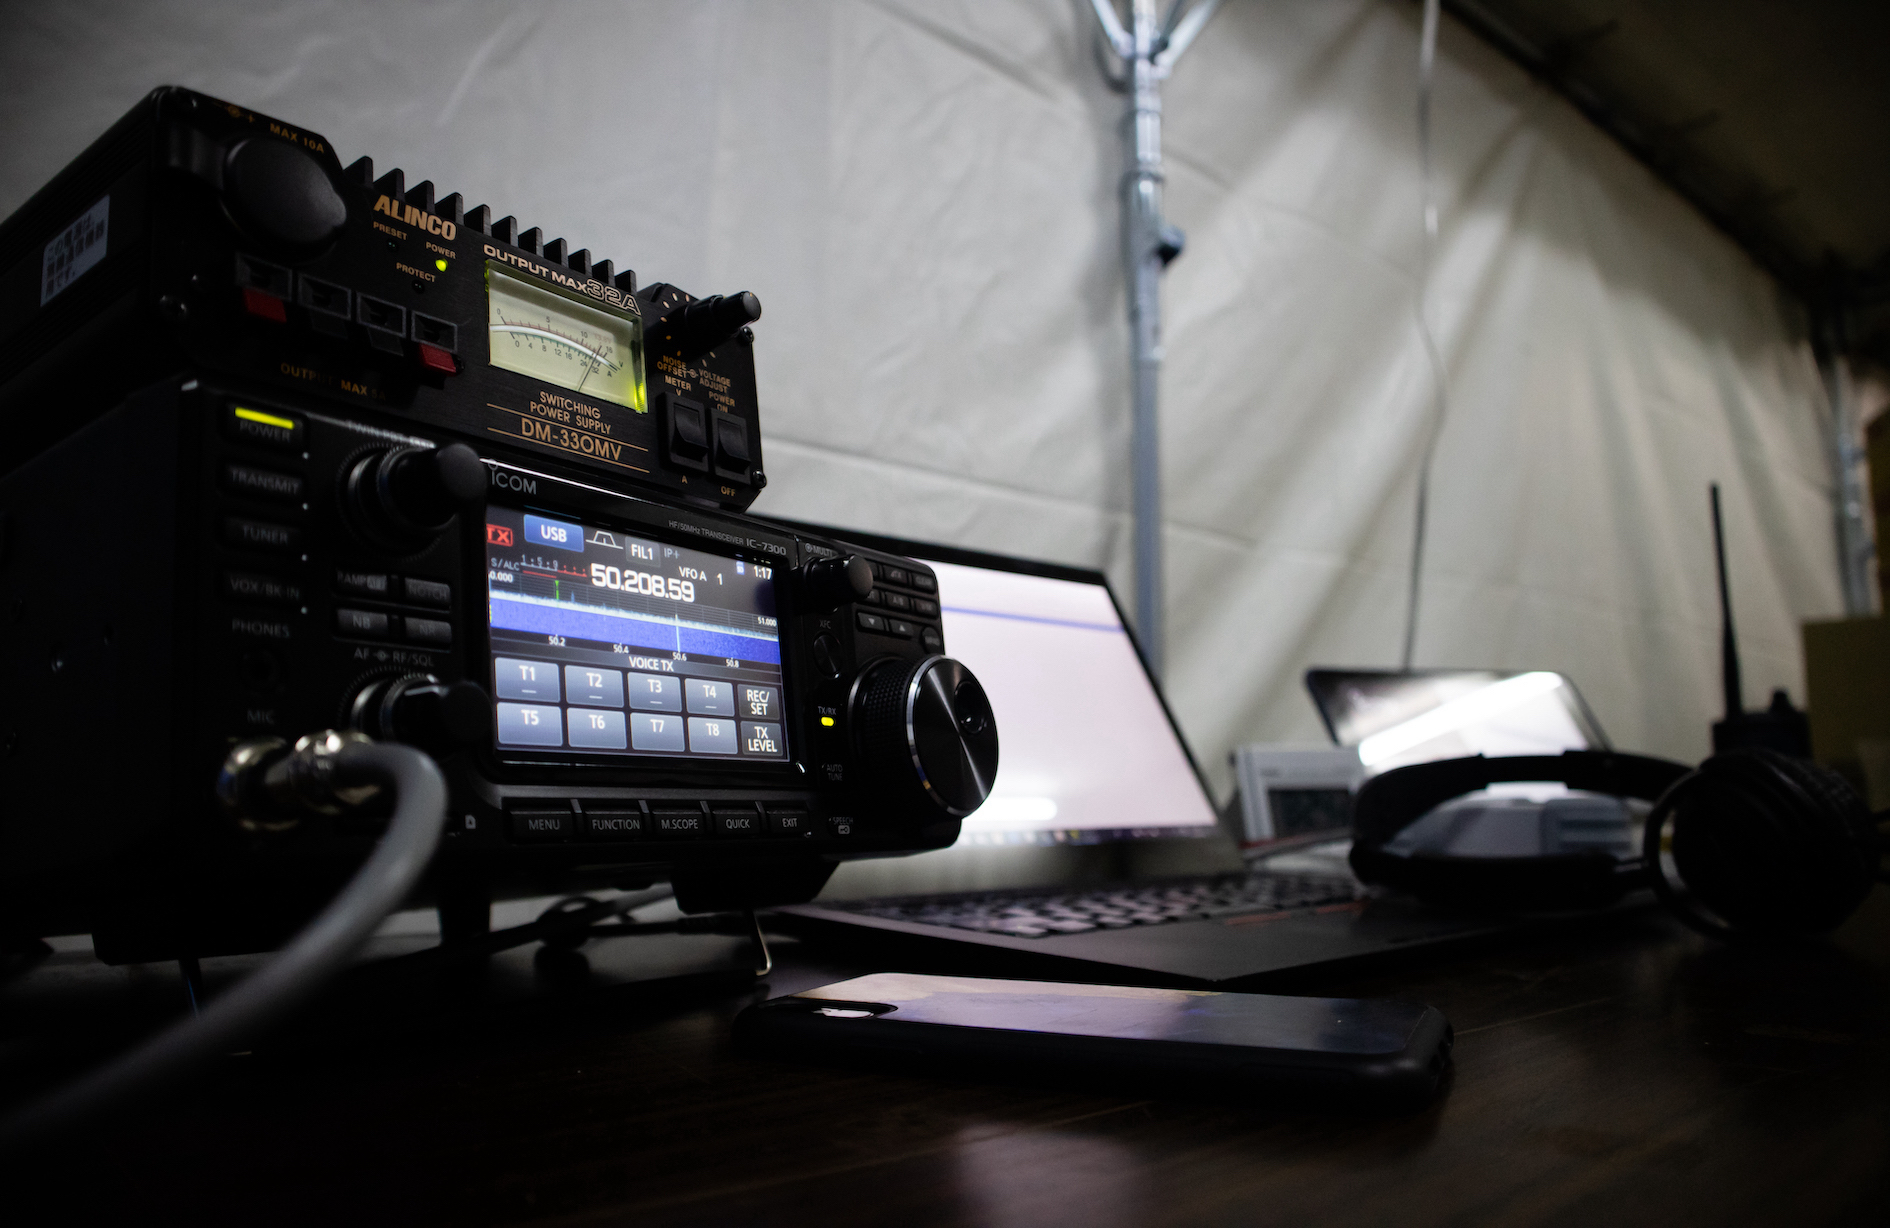
\includegraphics[width=.9\hsize]{pic/pic5.JPG}
                \end{center}
                % \caption{下宿先でフランベする図}
                % \label{fig:pic1}
            \end{figure}
        \end{column}
        \begin{column}{0.48\textwidth}
            \begin{figure}[htbp]
                \begin{center}
                    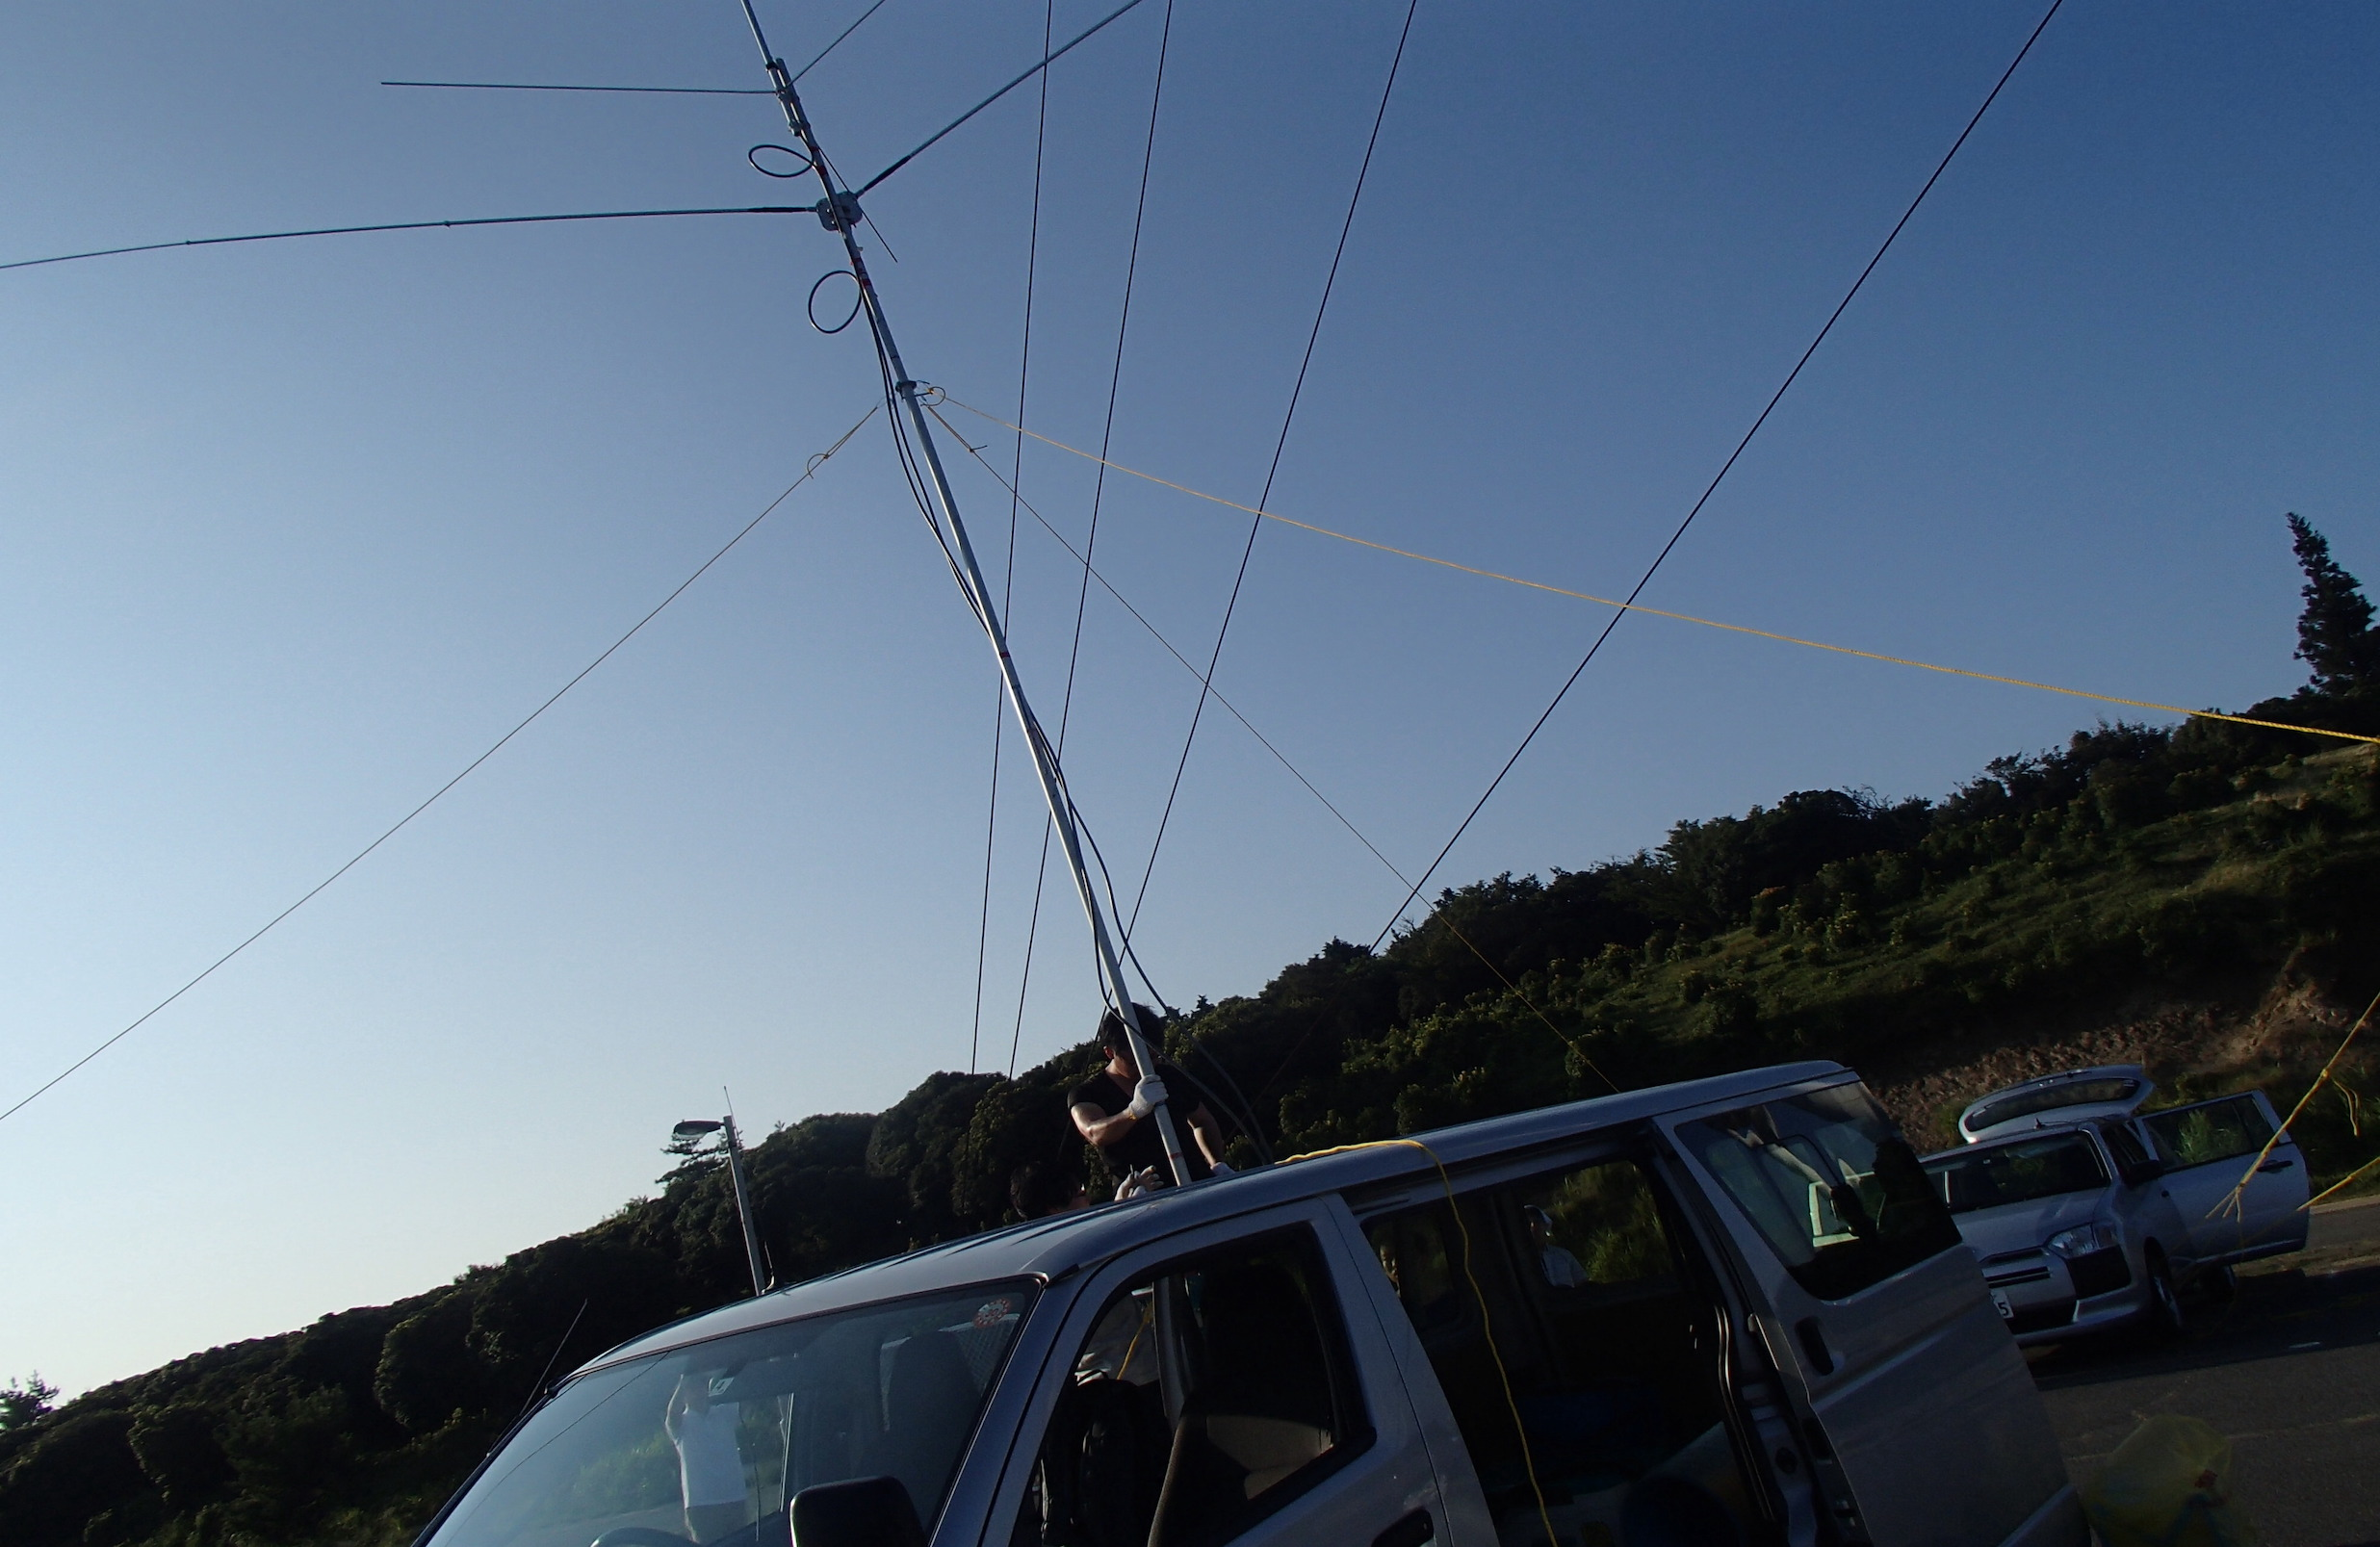
\includegraphics[width=.9\hsize]{pic/pic6.JPG}
                \end{center}
                % \caption{自家製ベーコン}
                % \label{fig:pic2}
            \end{figure}
        \end{column}
    \end{columns}
\end{frame}

%%% Local Variables:
%%% mode: japanese-latex
%%% TeX-master: "kosuge_slide"
%%% End:
